\vspace*{1pc}

The momentum of a photon is the frequency of its wave packet in units of $\hbar$. The FRW metric encoding the geometry of the expanding Universe is a troublesome system of coordinates because it is not linked to an inertial frame of reference. As such, the conservation of energy expressed by the Friedmann equations only hold for a fluid \emph{at rest} in the comoving coordinate system. Free-falling photons (\textit{i.e.} when not being absorbed), are constantly mobile in this coordinate system. On distances negligeble with respect to its proper time (its comoving particle horizon), photons occupy more or less the same comoving coordinate and nothing drastic or unexpected happens. On distances comparable to its proper time however, the photon's momentum is drained by the very geometry of the spacetime in which it is moving, given by expression~\ref{eq:momentum_ur}. Just as non-inertial reference frames see the spawning of fake centrifugal forces, the non-inertial nature of the comoving coordinate system has the consequence of \emph{not} conserving energy. Energy \emph{is} conserved in a fake so-called comoving volume, which can be thought of as the volume that expands (or contracts) homogenously with $a^3$. This is precisely what the cosmological redshift entails: a property of comoving observers and not of space. Neglecting the source's gravitational potential and its peculiar velocity with respect to the Hubble flow, the wavelength of the photon as measured by an observer is redshifted by the amount given in the defining relation~\ref{def:redshift}. Since the wavelength of the photon is the inverse of its Boltzmann temperature in units of $\hbar c/k_b$, it follows that the background teperature scales inversely with the scale factor.
\begin{equation}
\begin{array}{c}
\lambda(t) = \cfrac{\hbar c}{k_b T(t)} \propto a(t)\\
\Leftrightarrow\\
T(t) = T_0 \times \cfrac{a_0}{a(t)} = T_0 \times (1+z)
\end{array}
\end{equation}
Just as we've been introduced to the Friedmann equations as the Navier Stokes equations of a fluid at rest in the comoving coordinate system, let us venture into the thermodynamics of the Universe's contents in a comoving volume (sometimes called a covolume) where the temperature scales like $T(t) \propto a^{-1} (t)$.\\


\subsection{Maxwell Statistics}

Any interaction is maintained as long as its rate $\Gamma_{\mathrm{int}} \gg H$ overcomes the rate of expansion. This is the condition for any interaction to be at equilibrium in the expanding Universe. When $\Gamma_{\mathrm{int}} \lesssim H$, the interaction can no longer be maintained and the reactants decouple. In this section, I define all the relevant thermodynamical quantities that define the equilibrium state of any species thermalized with the background photons. The decoupling and production are dealt with in Sec.~\ref{sec:inventory}. The spatial homogeneity and isotropy of the background ensures $f$ is a function of only the magnitude of momentum and time. Absorbing the time dependance into the comoving momentum, one can write
\begin{equation}
f(\vec{x}, \vec{p}, \tau) = f(\vert \vert \vec{p} \vert \vert, \tau) = f(p, \tau) = f(q)
\end{equation} 

When in equilibrium, the distribution function of a particle of temperature $T = \alpha T_\gamma$ will obey either Fermi-Dirac statistics if it is made of fermions (baryons, neutrinos, and we'll assume dark matter) which feature the ``plus'' sign in the denominator of Eq.~\ref{eq:fermibose} or Bose-Einstein statistics if it is made of bosons (photons) with a ``minus'' sign:
\begin{empheq}[box=\mymath]{equation}
\label{eq:fermibose}
f_0(q) = \cfrac{1}{e^{\alpha \left[ \epsilon(q) - \xi \right]} \pm 1}
\end{empheq} with $T$ in units of $k_b$ and $\xi = \mu / T$ the comoving chemical potential, linked to the internal energy defined in the first principle ( $dU = T dS - \mathcal{P} dV + \mu dN$ ). It translates the fact that to conserve energy, a change in internal energy will alter the system's volume $dV$, its entropy (or ``useful'' work) $dS$ and the number of particles $dN$ (if it isn't conserved). The sum of the chemical potentials of reactants equals that of the products in a reaction at chemical equilibrium. Since conjugate particle-antiparticle pairs annihilate into two photons, the sum of their chemical potentials must equal that of two photons, which is zero since photon number is not conserved and can be produced in $e^{-} + p^{+} \leftrightarrow e^{-} + p^{+} + \gamma$ for instance. For a chemical potential $\mu_{\nu_\ell}$ of a neutrino of lepton charge $\ell$, its lepton-conjugate antineutrino has the opposite chemical potential \\
\begin{equation}
\mu_{\bar{\nu_\ell}} = - \mu_{\nu_\ell}
\end{equation} \\

\subsection{Density and Pressure}

The number density (Eq.~\ref{eq:number_density}), energy density and pressure (the diagonal components of Eq.~\ref{eq:nrj_general}) of radiation and matter at equilibrium are obtained using the equilibrium distribution function $f_0$ in expression~\ref{eq:fermibose}: \\
\begin{equation}
\label{eq:moments}
\left\{
\begin{array}{l}
n = \cfrac{g}{a^4} \displaystyle \int \cfrac{d^3 q}{(2 \pi)^3}~ f_0(p)\\
\rho  = \cfrac{g}{a^4} \displaystyle \int \cfrac{d^3 q}{(2 \pi)^3}~ f_0(q) ~\times~ \epsilon(q) \\
\mathcal{P} = \cfrac{g}{a^4} \displaystyle \int \cfrac{d^3 q}{(2 \pi)^3}~ f_0(q) ~\times~  \cfrac{q^2}{\epsilon(q)}
\end{array}
\right.
\end{equation} \\ and so the stress-energy tensor of the cosmological fluid at equilibrium is fully determined by Eq.~\ref{eq:fermibose}. All that remains is to delineate whether the two main particular components (matter and radiation) are fermions or bosons.\\

$\star$ For relativistic matter, with $\zeta$ the Riemann Zeta function, the number density, energy density and pressure are \\

\begin{equation}
\label{eq:relmat}
\left\{
\begin{array}{l}

n_{r} = \cfrac{\zeta(3)}{\pi^2} g T^3 \times \left\{ \begin{array}{ll}
1 & \text{for bosons}\\
\cfrac{3}{4} & \text{for fermions}
\end{array}
\right. \\
\\
\rho_{r} = \cfrac{\pi}{30} g T^4 \times \left\{ \begin{array}{ll}
1 & \text{for bosons}\\
\cfrac{7}{8} & \text{for fermions}
\end{array}
\right. \\
\\
\mathcal{P}_r = \cfrac{\rho_r}{3}

\end{array}
\right.
\end{equation} \\ and hence the equation of state of radiation is therefore 

\begin{empheq}[box=\mymath]{equation}
\label{eq:wr}
w_r = 1/3
\end{empheq} \\ This applies to photons, neutrinos when $k_b T > m_\nu c^2$, free electrons when $k_b T > 0.5~\mathrm{MeV}$ and quarks when $k_b T > 1~\mathrm{GeV}$.  \\

$\star$ For non-relativistic matter, which includes dark matter, free electrons when $k_b T < 0.5~\mathrm{MeV}$, free protons when $k_b T < 1~\mathrm{GeV}$, massive neutrinos when $k_b T < m_\nu^{\mathrm{eff}} c^2$, atoms, molecules, stars, dust, galaxies, \textit{etc}:

\begin{equation}
\label{eq:NR}
\left\{
\begin{array}{l}
n_m = g ~\left( \cfrac{\zeta(3)}{\pi^2} \right)^{3/2} \times e^{-m/T}\\
\\
\rho_m \simeq m n_m \\
\\
\mathcal{P}_m = n_m k_b T = \rho_m \cfrac{k_b T}{m} = \rho_m \cfrac{\langle v^2 \rangle}{3}
\end{array}
\right.
\end{equation} \\ Thus the equation of state for non-relativistic matter is \\
\begin{empheq}[box=\mymath]{equation}
\label{eq:wm}
w_m \simeq \frac{\langle v^2 \rangle}{3 c^2} \ll 1
\end{empheq} \\ which I will conventionally approximate to zero. For a Nitrogen gas ($N_2$) at room temperature for instance, $w_{N_2} \sim 10^{-12}$.

\subsection{Entropy}

In my investigation into neutrino mass and neutrino dark matter, I consider neutrinos (either left-handed or right-handed) and thermal relics which are produced in the early Universe and relativistic at the time of their respective decoupling. It is useful to introduce the number of relativistic species in thermal equilibrium with photons $g_\star^{\mathrm{th}}$:
\begin{equation}
g_{\star}^{\mathrm{th}} (T) = \sum_{\mathrm{bose}} g_{\mathrm{bose}} + \frac{7}{8} ~\sum_{\mathrm{fermi}} g_{\mathrm{fermi}}
\end{equation} where bosons (labeled `bose') contribute as $1 \times$ their number of spin states while fermions (labeled `fermi') contribute as $7/8$ their number of spin states to the radiation density (see second line in Eq.~\ref{eq:relmat}). One can similarly introduce the number of relativistic species decoupled from photons:
\begin{equation}
g_{\star}^{\mathrm{dec}} (T) = \sum_{\mathrm{bose}} g_{\mathrm{bose}} \left( \frac{T_{\mathrm{bose}}}{T} \right)^4 + \frac{7}{8} ~\sum_{\mathrm{fermi}} \left( \frac{T_{\mathrm{fermi}}}{T} \right)^4 g_{\mathrm{fermi}}
\end{equation} These two quantities enable one to write the energy density of relativistic species as a Stefan Laws:
\begin{equation}
\rho_r = \frac{\pi^2}{30} \times \left( g_{\star}^{\mathrm{th}} + g_{\star}^{\mathrm{dec}} \right)~T^4
\end{equation} \\

\begin{figure}
\begin{center}
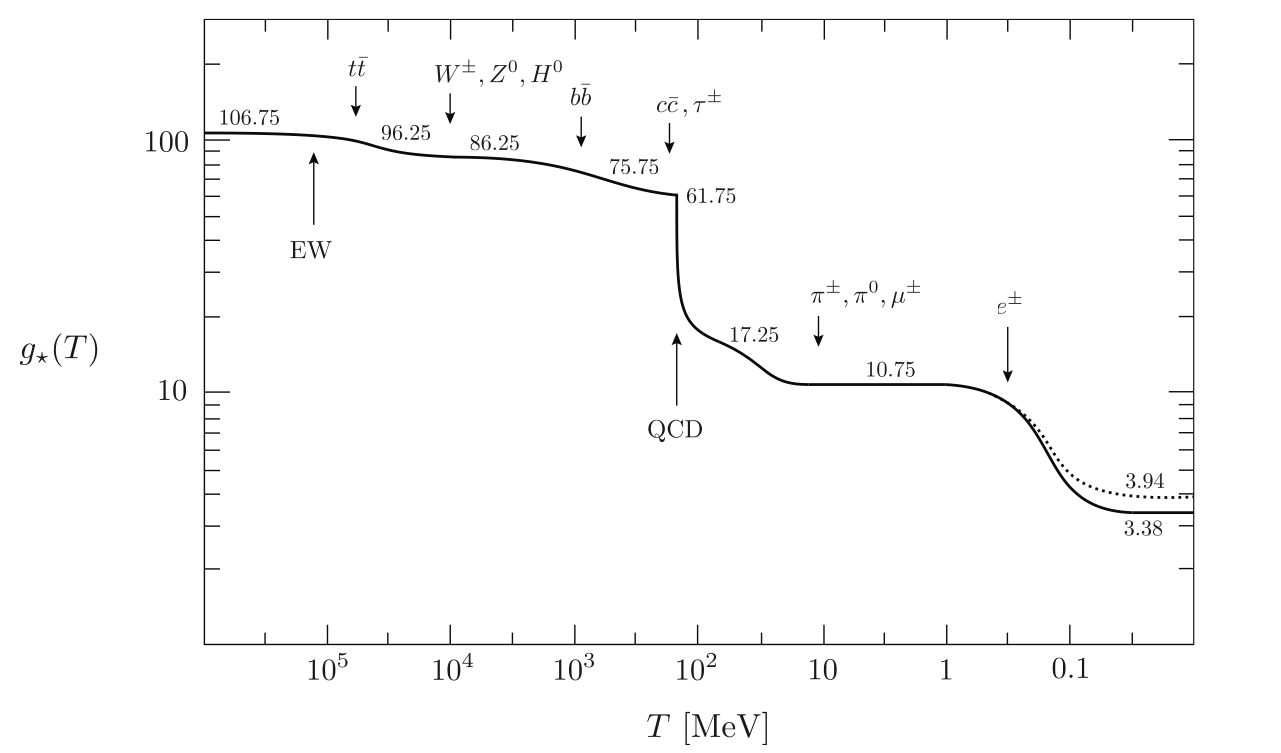
\includegraphics[width=\columnwidth]{Cosmology/gstar.png}
\end{center}
\caption{Effective number of relativistic degrees of freedom as a function of temperature. The numerical values are displayed before and after each phase transition. The solid line corresponds to $g_\star = g_{\star}^{\mathrm{th}} + g_{\star}^{\mathrm{dec}}$ whereas the dotted line corresponds to $g^s_{\star}$.}
\label{fig:gstar}
\end{figure}

The expansion of the Universe is often described as \emph{adiabatic}, which simply expresses that entropy is conserved, $dS / dT = 0$. The entropy density $s$ is defined as the sum of entropy densities of each species label by the index $\alpha$:
\begin{equation}
\label{eq:entropydensity}
s = \sum_{\alpha} \frac{\rho_{\alpha} + \mathcal{P}_{\alpha}}{T_{\alpha}} = \frac{2 \pi^2}{45} g^s_{\star} (T) T^3
\end{equation} where $g^s_{\star}$ is the effective number of degrees of freedom \emph{in entropy}. The entropy conservation assures that the entropy density scales as volume: $s \propto a^{-3}$, and so the temperature actually scales as $T \propto {g^s_\star}^{-1/3} a^{-1}$. Any relativistic species decoupling from the background photons alters the value of $g^s_\star$ and thus the evolution of the background temperature. Fig.~\ref{fig:gstar} recaps the value of $g_{\star}^{\mathrm{th}} + g_{\star}^{\mathrm{dec}}$ and $g^s_{\star}$ as a function of temperature.

\clearpage

